\documentclass[11pt, onecolumn]{article}
\usepackage{geometry}
\usepackage{graphicx}
\usepackage{amssymb}
\usepackage{microtype}
\usepackage{wrapfig}
\usepackage{amsmath}
\usepackage{indentfirst}
\usepackage{setspace}
\usepackage[format=plain, font=it]{caption}
\usepackage{todonotes}
\usepackage[hidelinks]{hyperref}
\usepackage{lipsum}

\geometry{a4paper, margin=2.5cm}
\singlespacing
\title{ES3J1 Group 3 Report}
\author{Anya Akram, Edward Stanley, Favour Rabiu, Matt Brooks, Nojus Plungė}
\date{\today}

\begin{document}
\pagenumbering{arabic}
\maketitle

\section*{Question 1}
\par INTRO
\par As the output produced by the motor is not smooth, to obtain its model that can be analysed using control system theory, a filter needs to be designed.
\\\par The filter (and thus, the model) tuning was done according to the brief provided for us. The process followed the steps outlined below:
\begin{enumerate}
    \item The filter coefficient was set to the simplest low-pass transfer function $\frac{1}{0.1s+1}$ to start smoothing the motor output, obtained by applying the step input. An example filter performance is shown in \textit{Figure \ref{fig:q1-filter}}.
          \begin{figure}[h!]
              \centering
              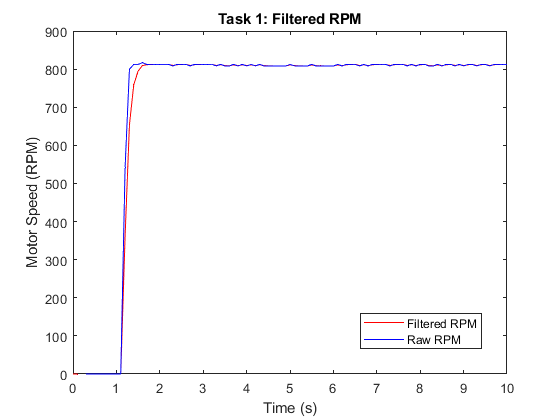
\includegraphics[width=0.5\textwidth]{q1-filter.png}
              \caption{Low-pass filter's impact on the signal.}
              \label{fig:q1-filter}
          \end{figure}
    \item The motor circuit, as set up in the brief, was assembled; the motor and Arduino were connected to the circuit and a link was established to the Simulink workspace.
    \item The motor was run using the MATLAB hardware add-on. The signal could be traced as going from the workspace input, through the PWM converter block and into the Arduino. The PWM signal generated by the Arduino then propagated through the circuit to power the motor, which had its encoder linked to the Arduino – this signal was then converted into motor RPM in the workspace and the obtained results were designated as the output. The input into the system and the output of the motor (in RPM) was saved to the workspace for further analysis.
    \item System Identification Toolbox (SIT) was used, with the input being the signal prior being processed by the PWM block and the output being the motor's revolutions per minute (RPM).
    \item In SIT the analysis was set for the transfer function to have no zeroes and one pole – this was chosen as the transfer function graph output from the unsmoothed output, by inspection, approximates to a first order transfer function output with step input.
    \item The obtained transfer function was scaled by dividing both the numerator and the denominator by step time.
    \item The obtained transfer function was plotted against the unfiltered motor output to verify the model accuracy and legitimacy. If proven significantly inaccurate, the design process was repeated until a fitting filter that produced a smooth transfer function was obtained.
\end{enumerate}
\par The resulting transfer function's step response is shown in \textit{Figure \ref{fig:q1-graph}} (titled as "Computed (SIT)"). \\\:
\par An alternative method for tuning the transfer function was also explored, as the steady state value of the produced function did not exactly match the motor output on the graph. The new tuning approach was found in \cite{umichControlTutorials} and was executed in the following steps:
\begin{enumerate}
    \item Steps 1-3 were repeated from the previous method: a simple low-pass filter was set up, motor circuit was assembled and the motor response to a step input was saved to the workspace.
    \item Find the maximum gain reached by the output. This will be regarded as the absolute – or steady state – gain. This was recorded to be a value of 834.
    \item The time constant for the response was calculated. As the first order transfer function subjected to a step response reaches 63.2\% of its output when the system reaches its first time constant. For this case, the value of 528.76 rpm needed to be reached – which the system does in 1.185s. As the step is applied at $t=1$ s, the time constant is $\tau = 1.185 - 1 = 0.185$s.
    \item Using the standard first order transfer function model:
          \begin{align*}
              G(s)=\frac{Y(s)}{X(s)}=\frac{K}{\tau s + 1}
          \end{align*}
          and substituting the values calculated, a final transfer function can be obtained:
          \begin{align*}
              G(s)=\frac{834}{0.185s + 1}
          \end{align*}
\end{enumerate}
\par The resulting transfer function's step response is shown in \textit{Figure \ref{fig:q1-graph}} (titled as "Graphical").
\begin{figure}[h!]
    \centering
    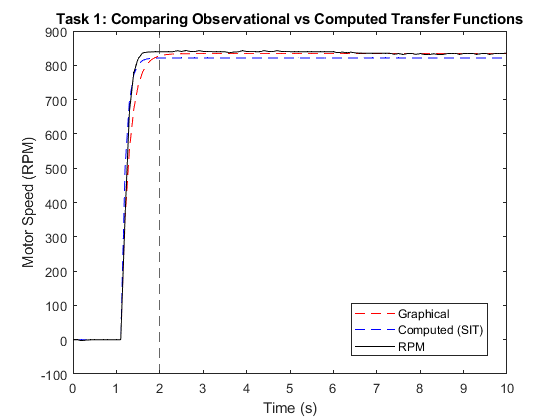
\includegraphics[width=0.6\textwidth]{q1-graphs.png}
    \caption{Step responses of transfer functions }
    \label{fig:q1-graph}
\end{figure}
\par The performance of the both functions were compared by calculating the mean-squared errors (MSEs) $\epsilon$ for each in a given timeframe:
\begin{itemize}
    \item Transient-state error ($0 < t <= 2$): the computed transfer function MSE was found to be $\epsilon_{ts-c} = 3.77 \times 10^4$, while the graphically-found transfer function's MSE was found to be $\epsilon_{ts-g} = 1.66 \times 10^4$. Overall, the MSE is 227\% higher on the SIT-computed than the graphically-calculated transfer function.
    \item Steady-state error ($t > 2$): the computed transfer function's MSE during the steady-state operation was found to be $\epsilon_{ss-c} = 243.0$ and the graphically-found transfer function's MSE during steady-state operation was $\epsilon_{ss-g} = 17.6$. Overall, there was a 1381\% increase in the MSE value of the SIT-calculated transfer function compared to the graphically-calculated transfer function.
    \item Overall error ($t > 0$): the total MSE for the SIT-calculated transfer function was $\epsilon_{T-c}=3.94\times10^{3}$ while the overall MSE for the graphically-calculated transfer function was $\epsilon_{T-g}=1.66\times10^{3}$. Overall, the total MSE was 237\% larger for the SIT-calculated transfer function than for the graphically-generated function.
\end{itemize}
\par Having evaluated the errors, any further tasks were performed using the graphically-generated transfer function, as it outperformed the SIT-generated function on every timeframe and fit the specifications just as well.
\par The final design allowed for the produced output to be of a smooth 1st order transfer function response, which enabled further analysis and tuning of the system in the subsequent tasks.
\section*{Question 2}
\par \textit{Describe all the steps that you used in obtaining the PI controller gains, (i.e. $K_p$ and $K_i$). It is highly encouraged to implement the PI controller manually instead of using the built-in PID Controller block.}
\par \textit{Include any results you deem essential to support your findings. Remember to take into practical consideration of the final controller gains that you will implement on the Arduino Uno. In other words, while in simulation, you can set the gains to a large value to get good performance, whether this large gain values are feasible or not to be implemented on the Arduino Uno is another matter.}
\noindent\makebox[\linewidth]{\rule{\textwidth}{0.4pt}}
\par \textbf{TEXT GOES HERE}
\section*{Question 3}
\par \textit{To fully test the performance of your PI controller, the Desired Motor Speed (Reference) should cover a substantial range of practical motor speed. Critically comment on your results. Include any results you deem essential to support your findings. Also, do remember to comment on the expectation (Task 2) versus reality (Task 3) of the implementation.}
\noindent\makebox[\linewidth]{\rule{\textwidth}{0.4pt}}
\par \textbf{TEXT GOES HERE}
\section*{Question 4}
\par \textit{Using what you have learned throughout this module (and beyond such as non- linearities effect, etc), try to improve the performance of the DC motor whether from the modelling side or the control design side. Feel free to explore and be adventurous in this exercise (as long as the safety precaution is adhered to ensure you do not damage the DC motor and the Arduino Uno). If required, revisit back all the steps from Tasks 1 to 3. Remember that in an actual engineering work, there is always room for improvement and the process is always iterative.}
\noindent\makebox[\linewidth]{\rule{\textwidth}{0.4pt}}
\par \textbf{TEXT GOES HERE}
\bibliographystyle{IEEEtran}
\bibliography{References}
\end{document}